\documentclass[border=10pt]{standalone}

\usepackage{tikz}
\usepackage{tikzsymbols}
\usetikzlibrary{calc,patterns,shapes.geometric}

\def\centerarc[#1](#2)(#3:#4:#5){\draw[#1] ($(#2)+({#5*cos(#3)},{#5*sin(#3)})$) arc (#3:#4:#5);}

\begin{document}
	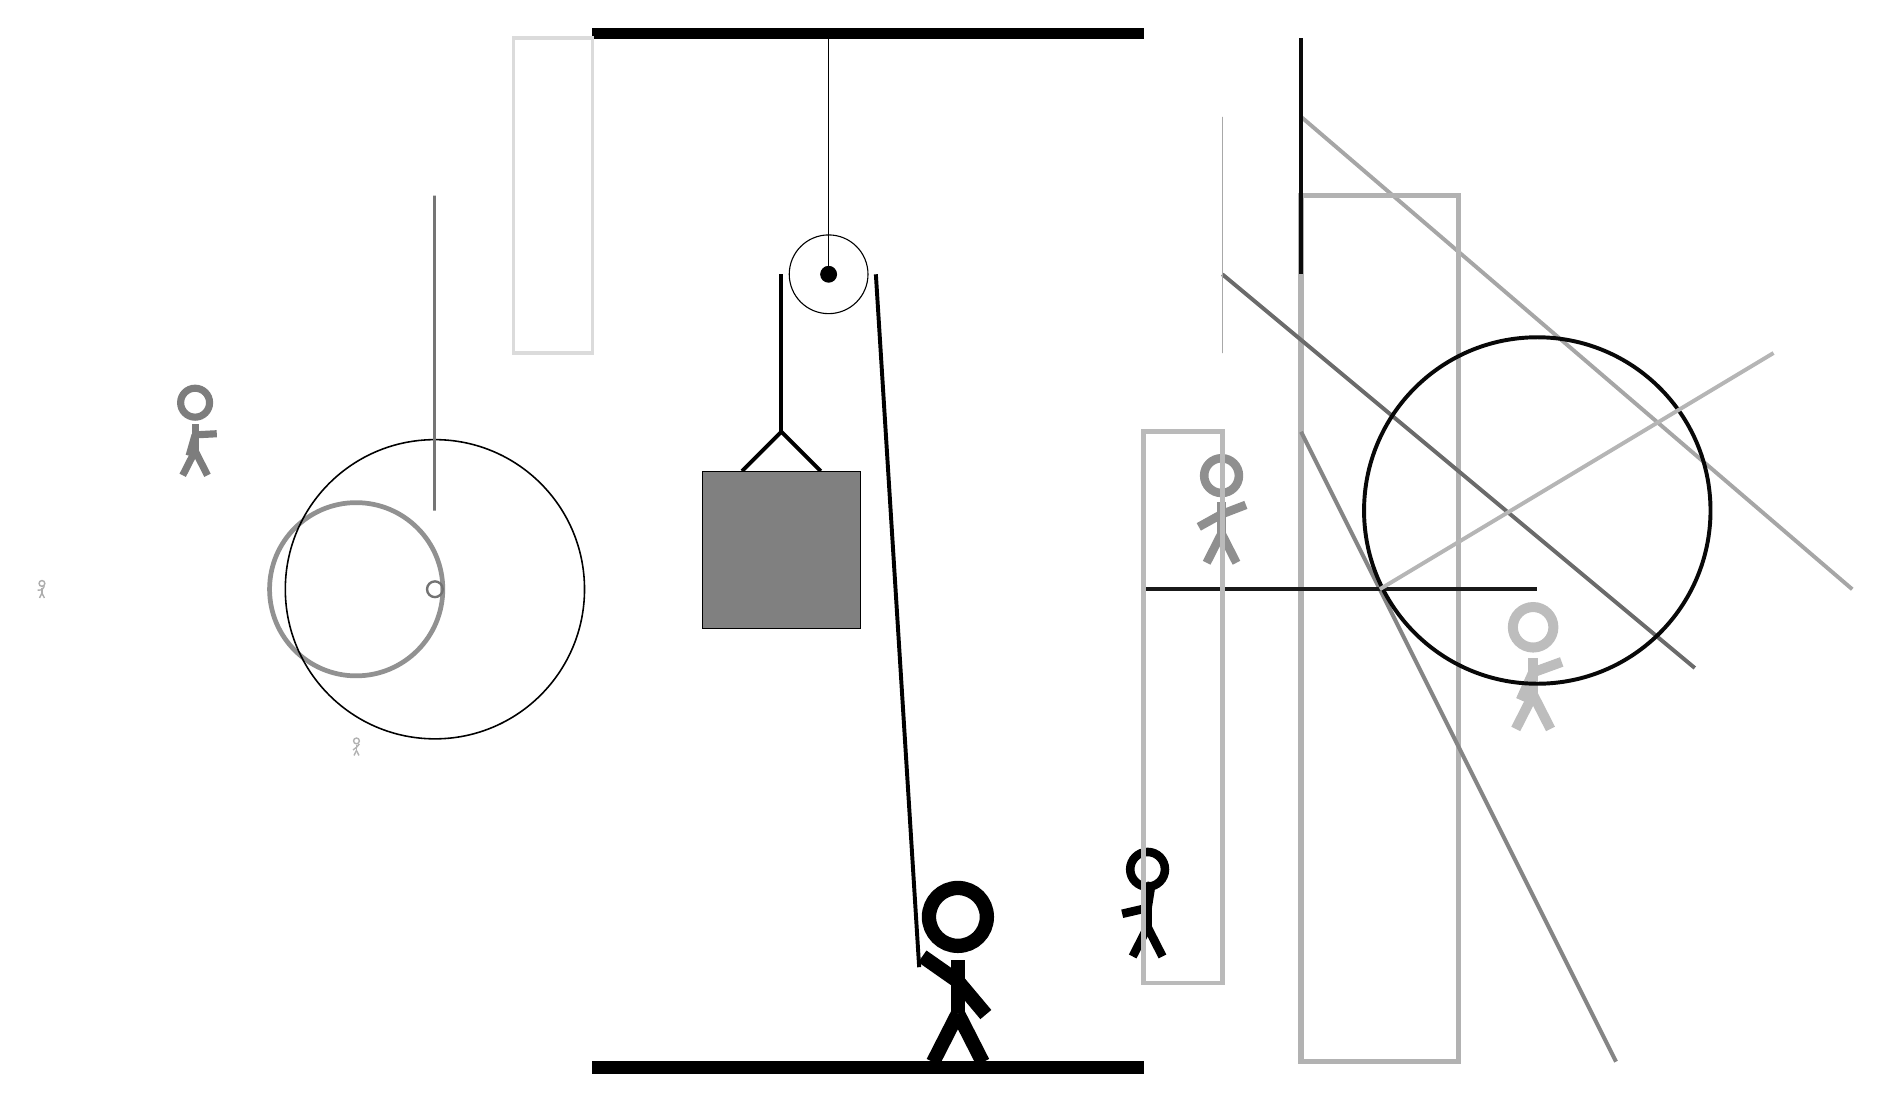
\begin{tikzpicture}
		%%%%% START %%%%%
		
		\draw[fill=black] (-2, 10) rectangle (5, 10.125);
		
		\draw (1, 7) circle (0.5);
		\draw[fill=black] (1, 7) circle (0.1);
		\draw (1, 10) -- (1, 7);
		
		\draw[line width=0.5mm] (-0.1, 4.5) -- (0.4, 5.0) -- (0.9, 4.5);
		\draw[fill=black!50] (-0.6, 4.5) rectangle (1.4, 2.5);
		
		\draw[line width=0.5mm] (0.4, 7) -- (0.4, 5.0);
		\centerarc[line width=0.5mm](1, 7)(0:180:0.6);
		\draw[line width=0.5mm](1.6, 7) -- (2.15, -1.8);
		
		\node[line width=0.6mm, color=black!44] at (6, 4) {\Strichmaxerl[6][29][21]};
		
		\draw[line width=0.5mm, color=black!35](7, 9) -- (14, 3);
		\draw [line width=0.6mm, color=black!43](-5, 3) circle (1.1);
		\node[line width=0.6mm, color=black!26] at (10, 2) {\Strichmaxerl[7][66][20]};
		\draw[line width=0.7mm, color=black!30] (7, -3) rectangle (9, 8);
		
		\draw[line width=0.5mm, color=black!48](7, 5) -- (11, -3);
		\draw[line width=0.5mm, color=black!58](6, 7) -- (12, 2);
		\draw [line width=0.2mm, color=black!100](-4, 3) circle (1.9);
		\draw[line width=0.5mm, color=black!90](5, 3) -- (10, 3);
		\draw [line width=0.5mm, color=black!97](10, 4) circle (2.2);
		\draw[line width=0.2mm, color=black!34] (6, 6) rectangle (6, 9);
		\draw[line width=0.5mm, color=black!29](8, 3) -- (13, 6);
		\node[line width=0.3mm, color=black!100] at (5, -1) {\Strichmaxerl[6][13][81]};
		
		\node[line width=0.3mm, color=black!32] at (-9, 3) {\Strichmaxerl[1][4][56]};
		\draw[line width=0.6mm, color=black!27] (5, -2) rectangle (6, 5);
		\draw[line width=0.4mm, color=black!54] (-4, 4) rectangle (-4, 8);
		\draw[line width=0.5mm, color=black!96](7, 10) -- (7, 7);
		
		\node[line width=0.6mm, color=black!30] at (-5, 1) {\Strichmaxerl[1][37][50]};
		\draw[line width=0.4mm, color=black!14] (-3, 6) rectangle (-2, 10);
		
		\node[line width=0.6mm, color=black!51] at (-7, 5) {\Strichmaxerl[5][74][3]};
		\draw [line width=0.3mm, color=black!55](-4, 3) circle (0.1);
		
		
		\node at (2.6, -1.9) {\Strichmaxerl[10][-35][-50]};
		
		\draw[fill=black] (-2, -3) rectangle (5, -3.15);
		
		%%%%% END %%%%%
	\end{tikzpicture}
\end{document}